\documentclass[dvipdfmx,uplatex]{jsarticle}
\def\vector#1{\mbox{\boldmath $#1$}}
\usepackage{qexam} % 問題を書く時とかに必要なやつ
\usepackage{setspace} % 行間開けるのに必要なやつ
\usepackage{amsmath} % 数学やるのに必要なやつ
\usepackage{bm} % 太字にするのに必要なやつ
\usepackage{amssymb}
% 画像を取り込むときに必要なやつ
\usepackage[dvipdfmx]{graphicx}
%\begin{figure}[htbp]
%\begin{center}
%\includegraphics[width=10cm]{フルパス}
%\caption{浜辺美波}
%\end{center}
%\end{figure}

\usepackage{ascmac}
\usepackage{siunitx}
\usepackage{float}
\usepackage{tikz}
\usepackage{circuitikz}
\usepackage{url}
\usepackage{braket}
\usepackage[colorlinks=true, bookmarks=true,
bookmarksnumbered = true, bookmarkstype = toc, linkcolor = black,
urlcolor=black, citecolor=black]{hyperref}
\usepackage{listings,jvlisting} % 日本語のコメントアウトをする場合jvlisting(もしくはjlisting)が必要
\lstset{
  basicstyle={\ttfamily},
  identifierstyle={\small},
  commentstyle={\smallitshape},
  keywordstyle={\small\bfseries},
  ndkeywordstyle={\small},
  stringstyle={\small\ttfamily},
  frame={tb},
  breaklines=true,
  columns=[l]{fullflexible},
  numbers=left,
  xrightmargin=0zw,
  xleftmargin=3zw,
  numberstyle={\scriptsize},
  stepnumber=1,
  numbersep=1zw,
  lineskip=-0.5ex
}%ここまでがプログラムのソースコードを貼るのに必要なやつ
\makeatletter
 \renewcommand{\theequation}{
   \thesubsection.\arabic{equation}}
  \@addtoreset{equation}{subsection}
\title{数値解析 授業まとめ}
\author{1019163 日置竜輔 \thanks{公立はこだて未来大学 システム情報科学部 複雑系知能学科 複雑系コース B3}}
\date{\today}

\begin{document}
\begin{spacing}{1.4}

\maketitle
\tableofcontents %目次

\newpage

\section{Pythonの標準入出力}
\begin{center}
  2021年4月13日 \\
\end{center}
省略
\newpage

\section{2分法・ニュートン法}
\begin{center}
  2021年4月20日 \\
\end{center}

\begin{quote}
 \begin{itemize}
  \item 2分法はニュートン法と比べると圧倒的の遅い。
 \end{itemize}
\end{quote}

\subsection{2分法で解が求められるか}
\begin{eqnarray}
  f(x) = (x - 1)^2 = 0の解が求められるかどうかを考察せよ。
\end{eqnarray}

A. 中間値の定理は任意の実数 $a$, $b$ に対して、$f(a) < 0 , f(b) > 0$となる点が存在することが十分条件である。 \\
しかし、任意の実数 $x$ に対して関数 $f(x)$ は $f(x) > 0$であるので、中間値の定理を用いることが出来ない。 \\
よって、中間値の定理を用いて、解を求める2分法は使用することが出来ない。

\subsection{ニュートン法の計算例}
\begin{eqnarray}
  e^{-x} - x^2 = 0はニュートン法で求めることが可能
\end{eqnarray}
\newpage

\section{ラグランジュ補間}
\begin{center}
  2021年4月27日 \\
\end{center}

\subsection{ラグランジュ補間の問題点}
補間の点数が増えてくると、ラグランジュの補間の近似の精度が悪くなることがある。\\これから、補間の関数が振動し、端の方ではかなり精度が悪いことがわかる。ラグランジュの補間では、補間の点数が増えてくると大きな振動が発生して、もはや補間とは言えなくなることがある。\\
ラグランジュの補間には常にこの危険性が付きまとうので、データ点数が多い場合は良い方法ではない。ほかの補間を選択しなくてはならない。

\begin{figure}[htbp]
\begin{center}
\includegraphics[width=7cm]{/Users/ryusuke/Documents/git/tex/NumericalAnalysis/img/ラグランジュ.png}
\caption{ラグランジュが端でバグるサンプル}
\end{center}
\end{figure}

\newpage

\section{スプライン補間}
\begin{center}
  2021年5月11日 \\
\end{center}
ラグランジュの補間はデータ点数が増えてくると関数が振動し,補間の精度が悪くなるのは先に述べた
とおりである.そこで,補間する領域をデータ間隔 $[xi, xi+1]$ に区切り,その近傍の値を使い低次の多項式で近似することを考える.\\
区分的に近似関数を使うわけですが,上手に近似をしないと境界でその導関数が不連続になる.導関数が連続になるように,上手に近似する方法がスプライン補間 (spline interpolation)である.\\
ここでは,通常よくつかわれる 3 次のスプライン補間について説明する.補間する関数が 3 次関数を使うため,そう呼ばれている.これ以降の説明は,文献 [1] を参考にした.\\
データは先と同じように $(x0, y0),(x1, y1), (x2, y2), ... , (xN , yN )$ とする.そして,区間 $[xj , xj+1]$ で補間に使う関数を Sj (x) とする.この様子を図 5 に示す.

\begin{figure}[htbp]
\begin{center}
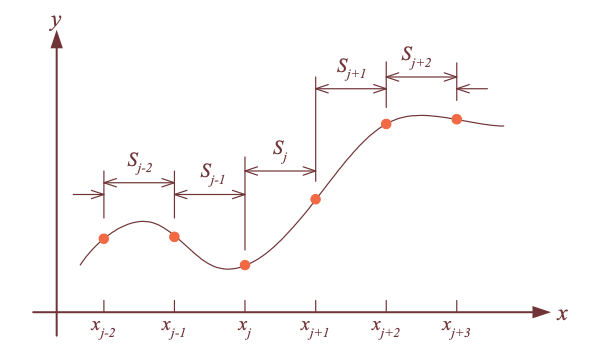
\includegraphics[width=7cm]{/Users/ryusuke/Documents/git/tex/NumericalAnalysis/img/スプライン補間.png}
\caption{スプライン補間の区分}
\end{center}
\end{figure}

\subsection{ラグランジュ補間とスプライン補間の違い}
ラグランジュ補間では,データによっては意図しない形状になることがある.(4次関数なので,関数の両端が上昇か下降かのどちらかにしかならない.)\\
例えば,周期関数や指数関数,正規分布など,必ずしも多項式での近似がふさわしくない場合がある.\\
そこで,与えられた点群すべてを使って関数を決定するのではなく,局所的な数点のみを使って局所の関数(曲線)を決定し,かつ,その曲線が全体として滑らかに接続されるような補間法が広く利用されている.\\
その代表例がスプライン補間である.\\
スプライン補間では,点群全体から単一の多項式を求めるのではなく,「各区間」を次数の比較的低い多項式で近似する.\\
多項式にはいろいろ考えられるが,ここでは以下の3次式を用いる「3次のスプライン補間」を行う.

\newpage

\section{最小二乗法と連立一次方程式}
\begin{center}
  2021年5月18日 \\
\end{center}
最小二乗法で求めたい式は、
\begin{eqnarray}
  y = a_0x + a_1
\end{eqnarray}

\begin{quote}
 \begin{itemize}
  \item 最小二乗法は2乗誤差の総和を最小にするように係数$a_0, a_1$を定めること
 \end{itemize}
\end{quote}

\subsection{推定誤差}
\begin{eqnarray}
  e_i = y_i - (a_0x_i + a_1)
\end{eqnarray}

\subsection{2乗誤差の総和}
\begin{eqnarray}
  S &=& \sum_{i=1}^{k}e_i^2 = \sum_{i=1}^{k} \{y_i - (a_0x_i + a_1)\}^2 \\
    &=& a_0^2(\sum_{i=1}^{k} x_i^2) - 2a_1\{\sum_{i=1}^{k} x_i(y_i - a_1)\} + \sum_{i=1}^{k}(y_i - a_1)^2
\end{eqnarray}

みたいな感じになるのであとは適当に括って、最小化、つまり偏微分して0になるような点を求めれば良い。\\

\begin{quote}
 \begin{itemize}
  \item 連立1次方程式はガウスの消去法を用いると$O(N^3)$であるが、LU分解を用いると$O(N^2)$で収まるため、とても高速に処理することが可能となる。
 \end{itemize}
\end{quote}
\newpage

\section{}
\begin{center}
  2021年5月25日 \\
\end{center}

\newpage

\section{}
\begin{center}
  2021年4月20日 \\
\end{center}

\newpage

\section{}
\begin{center}
  2021年4月20日 \\
\end{center}

\newpage

\section{}

\newpage

\section{}

\newpage

\end{spacing}
\end{document}
